% $Header: /cvsroot/latex-beamer/latex-beamer/solutions/generic-talks/generic-ornate-15min-45min.en.tex,v 1.5 2007/01/28 20:48:23 tantau Exp $

\documentclass{beamer}

% This file is a solution template for:

% - Giving a talk on some subject.
% - The talk is between 15min and 45min long.
% - Style is ornate.



% Copyright 2004 by Till Tantau <tantau@users.sourceforge.net>.
%
% In principle, this file can be redistributed and/or modified under
% the terms of the GNU Public License, version 2.
%
% However, this file is supposed to be a template to be modified
% for your own needs. For this reason, if you use this file as a
% template and not specifically distribute it as part of a another
% package/program, I grant the extra permission to freely copy and
% modify this file as you see fit and even to delete this copyright
% notice.


\mode<presentation>
{
  \usetheme{Antibes}
  \setbeamercovered{transparent}
}

\usepackage{graphicx}
\usepackage[english]{babel}
% or whatever

\usepackage[latin1]{inputenc}
% or whatever

\usepackage{times}
\usepackage[T1]{fontenc}
% Or whatever. Note that the encoding and the font should match. If T1
% does not look nice, try deleting the line with the fontenc.


\title[] % (optional, use only with long paper titles)
{Using ROS}
% \subtitle
% {Presentation Subtitle} % (optional)

\author[] % (optional, use only with lots of authors)
{Jeremiah Via}
% - Use the \inst{?} command only if the authors have different
% affiliation.

\date[] % (optional)
{23 February 2011}

\subject{Talks}
% This is only inserted into the PDF information catalog. Can be left
% out.

% Delete this, if you do not want the table of contents to pop up at
% the beginning of each subsection:
\AtBeginSubsection[]
{
  \begin{frame}<beamer>{Outline}
    \tableofcontents[currentsection,currentsubsection]
  \end{frame}
}

\begin{document}

\begin{frame}
  \titlepage
\end{frame}

\begin{frame}{Outline}
  \tableofcontents
  % You might wish to add the option [pausesections]
\end{frame}


% Since this a solution template for a generic talk, very little can
% be said about how it should be structured. However, the talk length
% of between 15min and 45min and the theme suggest that you stick to
% the following rules:

% - Exactly two or three sections (other than the summary).
% - At *most* three subsections per section.
% - Talk about 30s to 2min per frame. So there should be between about
% 15 and 30 frames, all told.

\section{What is ROS?}

\subsection{Basics}
\begin{frame}
  \begin{itemize}
  \item Robot Operating System
    \pause
  \item Meta-operating System
    \pause
  \item Originally developed in 2007 at Stanford AI Lab
    \pause
  \item Now developed at Willow Garage
  \end{itemize}
\end{frame}

\subsection{Vocabulary}

\begin{frame}{Node}
  \begin{itemize}
  \item A process that performs computation
  \end{itemize}

  \begin{figure}
    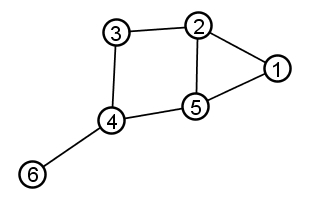
\includegraphics[scale=0.5,clip=true]{six-nodes.jpg}
  \end{figure}
\end{frame}

\begin{frame}{Message}
  \begin{itemize}
  \item The way nodes communicate to one another
  \item Strictly typed
  \end{itemize}

  \begin{figure}
    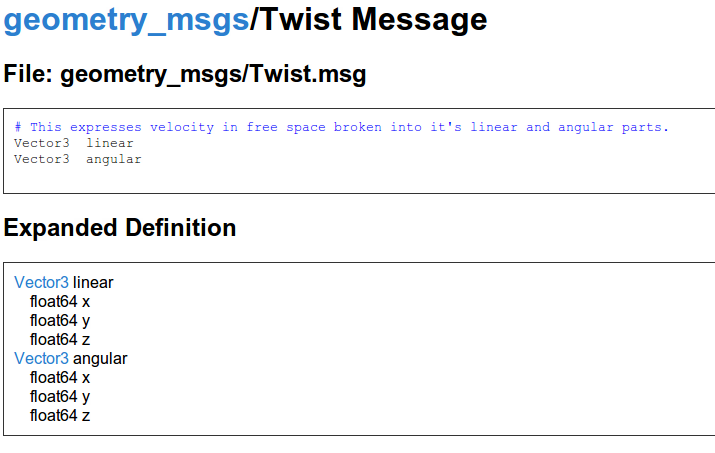
\includegraphics[scale=0.30]{geometry-message.png}
  \end{figure}
\end{frame}

\begin{frame}{Topic}
  \begin{itemize}
  \item String which labels a stream of data, \emph{e.g.},
    \texttt{cmd\_vel} or \texttt{scan}
  \item Nodes can subscribe and publish to these topics
  \end{itemize}

  \begin{figure}
    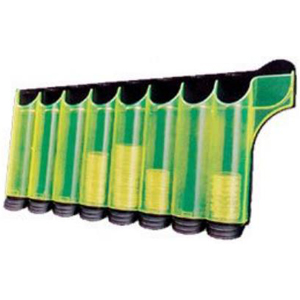
\includegraphics[scale=0.5]{coin_sorter_green.jpg}
  \end{figure}
\end{frame}

\begin{frame}{Service}
  \begin{itemize}
  \item Synchronous transaction (like a webpage request)
  \end{itemize}

  \begin{figure}
    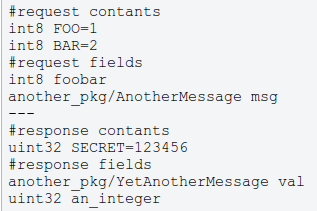
\includegraphics[scale=0.65]{service.png}
  \end{figure}
\end{frame}


\subsection{Architecture}
\begin{frame}{Peer-to-Peer}
  \begin{itemize}
  \item Designed to have many nodes running
  \item Communication is managed by the master node
  \end{itemize}

  \begin{figure}
    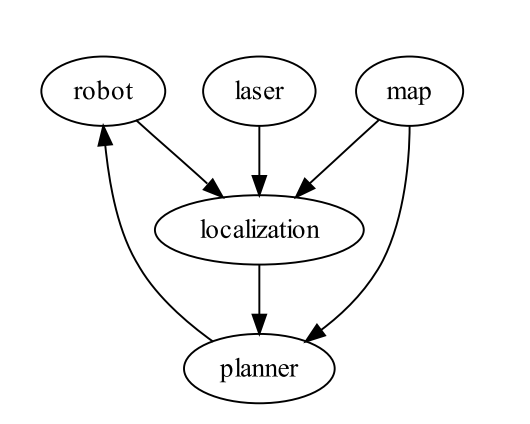
\includegraphics[width=5.0cm]{network_graph.png}
  \end{figure}
\end{frame}

\begin{frame}{Language Agnostic}
  \begin{figure}
    
\includegraphics[width=10cm]{lang-logo.png}
  \end{figure}
\end{frame}


\begin{frame}{Tools-based}
  \begin{itemize}
  \item Follows the UNIX philosophy of many small tools
  \item Less efficient but more stable and less complex
  \item Example tools
    \begin{itemize}
    \item \texttt{roscd}
    \item \texttt{rosls}
    \item \texttt{rosinstall}
    \item \texttt{rostopic}
    \item \texttt{roscreate-pkg}
    \end{itemize}
  \end{itemize}
\end{frame}


\begin{frame}{Thin}
  \begin{itemize}
  \item Algorithm and driver development occur as standalone libraries
  \item Small executables expose library functionality
  \end{itemize}

  \begin{figure}
    
\includegraphics[width=2.5cm]{opencv-logo.png}
  \end{figure}

  \begin{figure}
    
\includegraphics[width=2.5cm]{player-logo.png}
  \end{figure}
\end{frame}


\section{Why ROS?}
\subsection{Reasons}

\begin{frame}{Debugging}
  \begin{itemize}
  \item Debugging is hard \pause
  \item Debugging robots is really hard \pause
  \item Modular design
    \begin{itemize}
    \item Only need to restart the modified nodes
    \item Graph structure modified silently
    \item No need to take down the entire system
    \end{itemize}
  \end{itemize}
\end{frame}

\begin{frame}{Logging \& Playback}
  \begin{itemize}
  \item ROS can log any data we want it to \pause
  \item Logged data can be used to test various algorithms \pause
  \item Data can even be used to create a map
  \end{itemize}

  \begin{figure}
    
\includegraphics[width=5cm]{map.png}
  \end{figure}
\end{frame}

\begin{frame}{Packaged Subsystems}
  \begin{itemize}
  \item Some areas of research are mature enough to use standard
    algorithms
  \item No sense in reimplementing a new SLAM system for each new
    robot
  \item ROS allows multiple packages to be run together: \texttt{roslaunch}
  \end{itemize}
\end{frame}

\begin{frame}{Visualizations \& Monitoring}
  \begin{itemize}
  \item Printed data can be hard to understand \pause
  \item Printed data is impossible to understand when it's in 3D \pause
  \item ROS has a built-in tool to help visualize sensor data called rviz
  \end{itemize}

  \begin{figure}
    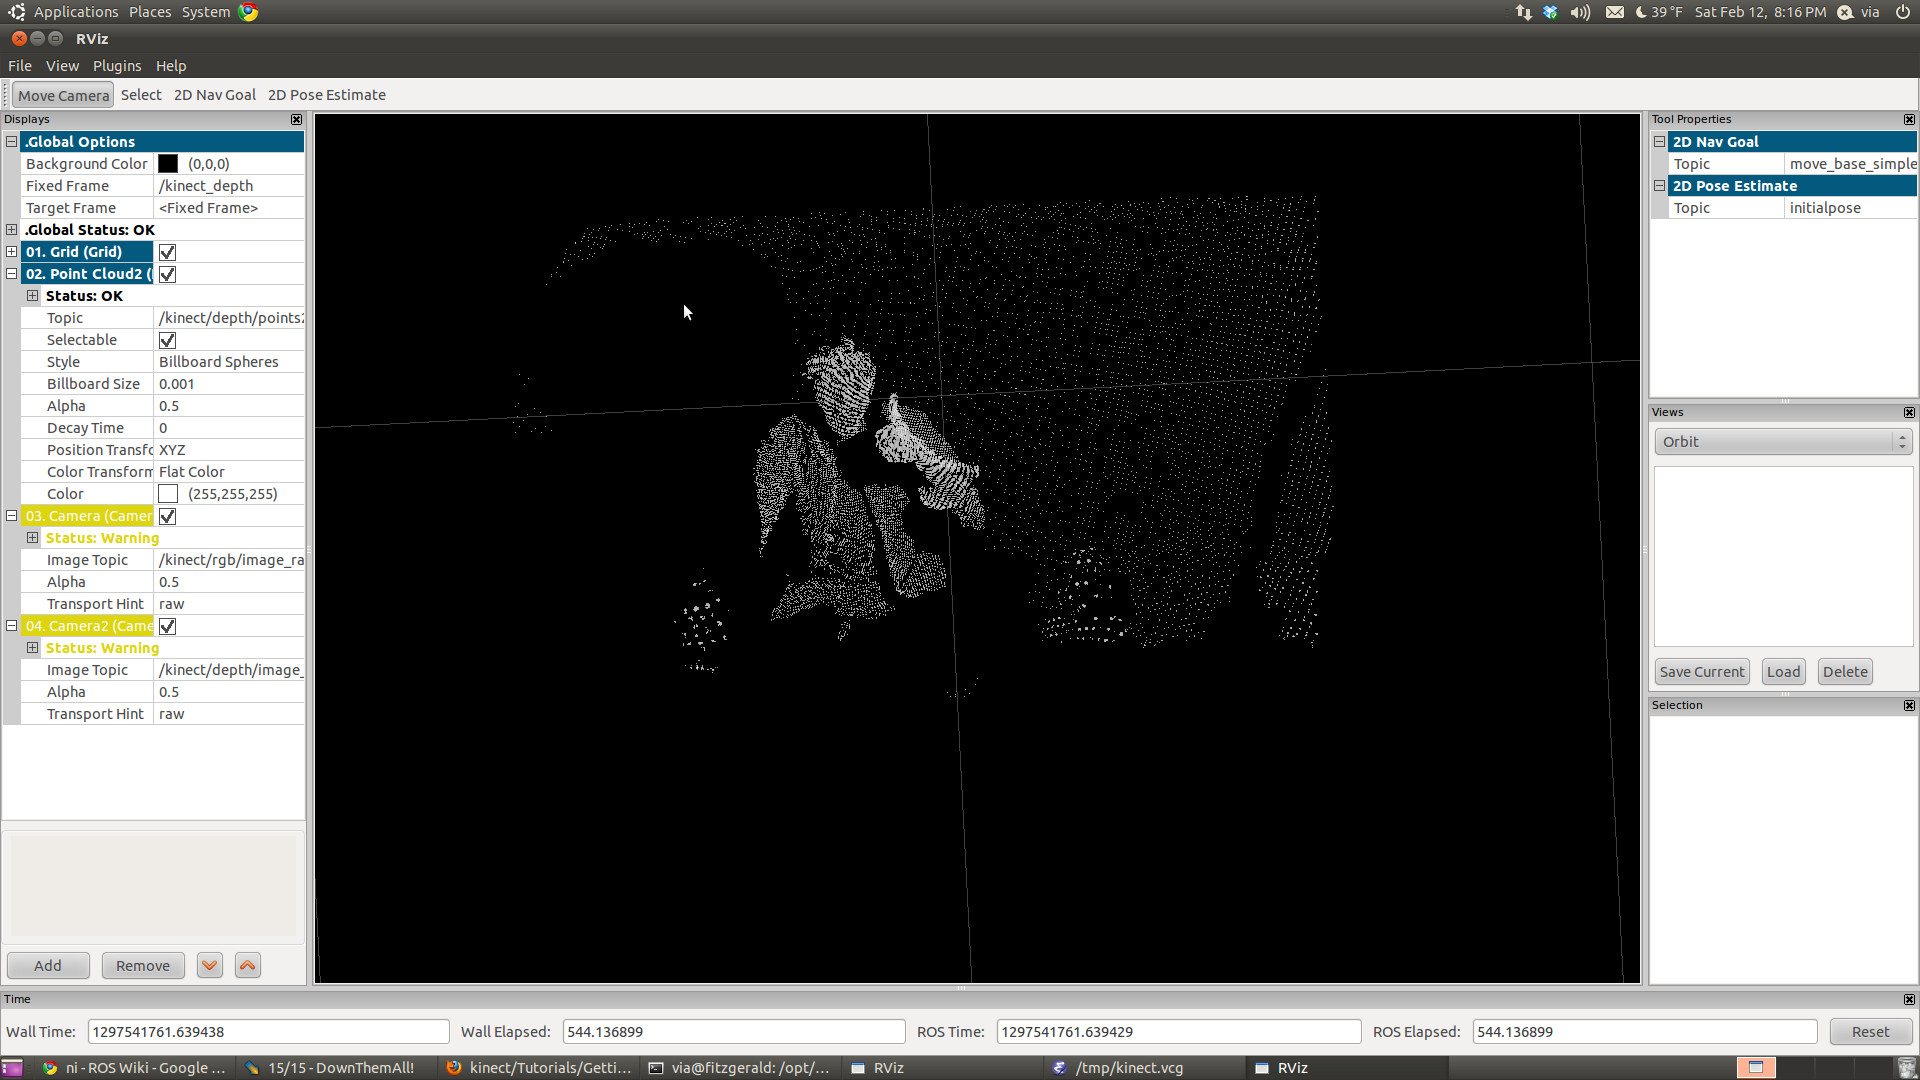
\includegraphics[trim = 0mm 30mm 0mm 0mm, clip, width=9cm]{rviz.png}
  \end{figure}
\end{frame}

\section{Code Example}
\subsection{Python}
\begin{frame}{Simple Python Example}
  Robot Programming Exercise 3 part 1:
  \begin{quote}
    Build a control strategy that keeps the robot a set distance
    away from an obstacle in front of it.
  \end{quote}
\end{frame}

\section{Getting Involved}
\subsection{Robot Club}

\begin{frame}{Join the Mailing List}

  \begin{itemize}
  \item The simplest way to get started is to join the mailing list
  \item \url{https://mailman.cs.bham.ac.uk/mailman/listinfo/robot-club}
  \end{itemize}
  
  \begin{figure}
    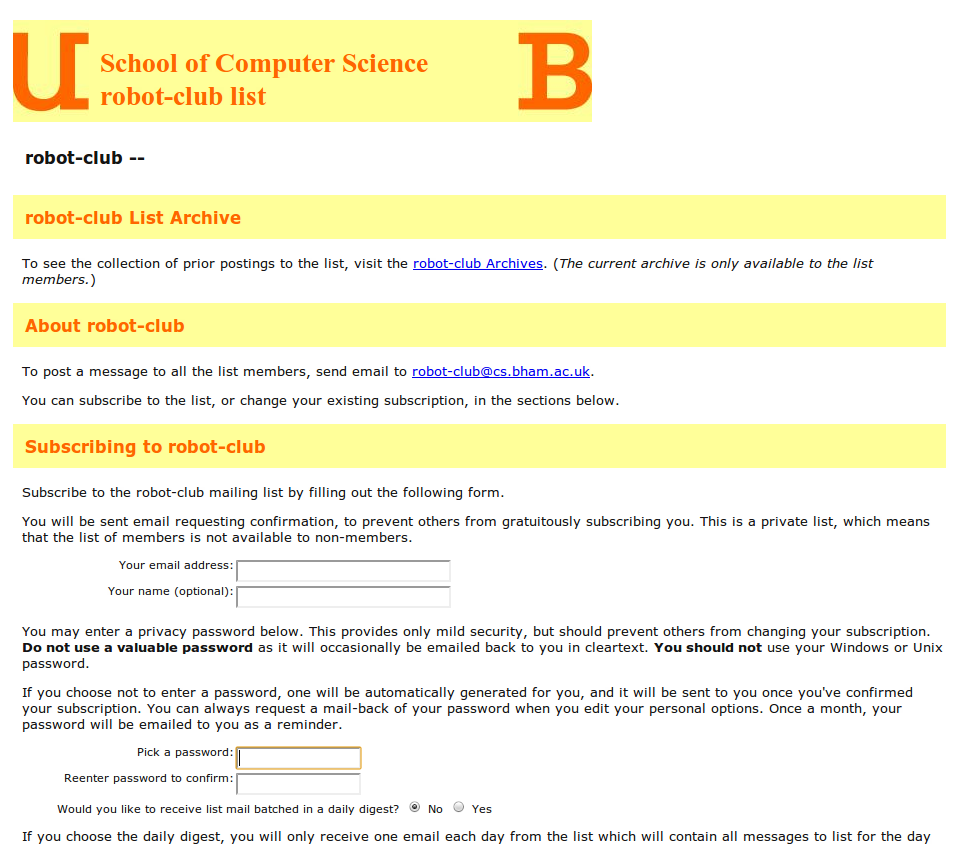
\includegraphics[width=7cm]{mailinglist.png}
  \end{figure}

\end{frame}

\begin{frame}{Install ROS} 
 
  \begin{itemize}
  \item Go to \url{http://www.ros.org/wiki/ROS/Installation} for
    installation instructions
  \end{itemize}

  \begin{figure}
    
\includegraphics[width=8cm]{os.png}
  \end{figure}

\end{frame}

\begin{frame}{Check out the Code}

  \begin{itemize}
  \item \texttt{svn checkout https://codex.cs.bham.ac.uk/svn/nah/robot club}
  \end{itemize}

\end{frame}

\section*{Summary}

\begin{frame}{Summary}

  \begin{itemize}
  \item ROS is powerful and useful
  \item Robot club is fun
  \item Join!
  \end{itemize}

\end{frame}

\end{document}


